\documentclass[journal]{IEEEtran}
\usepackage[T1]{fontenc}
\usepackage{lmodern}
\usepackage{amsmath,amssymb}
\usepackage{graphicx}
\usepackage{booktabs}
\usepackage{array}
\usepackage{multirow}
\usepackage{xcolor}
\usepackage{microtype}
\usepackage{url}
\usepackage[hidelinks]{hyperref}
\usepackage{cite}
\graphicspath{{figures/}}

\newcommand{\vuln}{\textsc{vulnerable}}
\newcommand{\safe}{\textsc{safe}}
\newcommand{\pc}{P-C@1}
\newcommand{\sd}{\ensuremath{\Delta}}

\hypersetup{pdftitle={Verifiable Rewards, Unverified Discrimination: Two Independent Instrumented Studies of GRPO for Paired C/C++ Vulnerability Detection},
pdfauthor={Dhruv Jyoti Das, T. Grace Shalini}}

\begin{document}

\title{Verifiable Rewards, Unverified Discrimination:\\
Two Independent Instrumented Studies of GRPO\\
for Paired C/C++ Vulnerability Detection}

\author{Dhruv Jyoti Das$^{*}$ and T. Grace Shalini$^{\dagger}$\\
$^{*}$Department of Computing Technologies, SRM Institute of Science and Technology, India\\
Email: dd4708@srmist.edu.in, ORCID: 0009-0002-8705-5962\\
$^{\dagger}$Department of Computational Intelligence, SRM Institute of Science and Technology, India\\
Email: gracesht@srmist.edu.in, ORCID: 0000-0002-0016-3702}

\markboth{Manuscript draft, compiled from the TraceGRPO and VulnGuard research records}{}
\maketitle

\begin{abstract}
We report two independently engineered, pre-registered programs that ask one question---does reinforcement learning with verifiable rewards (GRPO) create vulnerability \emph{discrimination} in a $\sim$4B-parameter code model on paired C/C++ functions?---and reach the same answer by different routes.
\textbf{Program A (TraceGRPO)} trains Qwen3-4B on a 27,314-row chronological corpus with a teacher-trace SFT cold start and a five-component reward. Three SFT variants learn the output contract (up to 99.68\% parse) yet score at chance (50.18--50.50\% accuracy); production GRPO leaves matched row AUC at $\le 0.5163$ with every paired interval including zero; a closed-form equilibrium $q^*=\kappa\Delta_V/(\kappa\Delta_V+\Delta_S)$ predicts the observed verdict-prior drift; a corrected balanced reward confirms its behavioral prediction yet misses its pre-registered discrimination target ($\Delta$AUC $-0.0077$ [$-0.0253$, $+0.0096$]).
\textbf{Program B (VulnGuard)} trains from the untrained base on 1,900 pairs with a gold reward against placebo rewards that permute, binarize or flip it. Gold-reward GRPO collapses to an always-\safe{} policy in every fresh matched seed (3/3) and in every historical credit-assignment variant; the permuted placebo drifts to \vuln{}. On 416 held-out pairs, strict localized pair-correctness is 0.06\% (gold) versus 1.10\% (permuted), a difference of $-1.04$\,pp [$-1.52$, $-0.62$]---and 4.30\% for the \emph{untrained} base. Two purpose-built rescues fail: a constrained verdict-rate clamp (always-\safe{}; its cost signal is exactly zero once a group collapses to one verdict) and a pair-symmetric reward (relocates collapse to always-\vuln{}).
Across both programs, every system lies on the no-discrimination diagonal of $(P(\vuln\mid\text{safe}),P(\vuln\mid\text{vulnerable}))$ space; RL moved the verdict prior, not the discrimination. We give reward-geometry accounts of the direction of that movement, list the claims the evidence does not support, and document corrections to earlier drafts of both studies.
\end{abstract}

\begin{IEEEkeywords}
Vulnerability detection, large language models, GRPO, reinforcement learning with verifiable rewards, reward hacking, policy collapse, placebo rewards, pre-registration, negative results.
\end{IEEEkeywords}

\section{Introduction}
\IEEEPARstart{L}{arge} language models are increasingly trained for vulnerability detection with supervised fine-tuning on teacher rationales and with reinforcement learning from verifiable rewards (RLVR), most often a GRPO-family objective~\cite{grpo,vulpo,openvul,r2vul,vulnllmr,simoni}. The implicit premise is that a programmatically checkable reward transmits the capability it measures. Two lines of work make that premise uncomfortable: spurious or even random rewards can produce RLVR gains on reasoning tasks~\cite{spurious}, and RL may resample rather than expand what the base model can do~\cite{yue,prorl}; meanwhile, vulnerability benchmarks are known to overstate detector quality once deduplication, chronology and paired evaluation are applied~\cite{primevul,risse,das}.

This paper joins two research programs that were built separately, on overlapping but not identical data, with different pipelines, and that were each run under frozen splits, pre-registered gates and self-executing stop rules:

\begin{itemize}
\item \textbf{Program A, TraceGRPO.} Joint detection, statement localization and source-to-sink trace explanation on a 27,314-row corpus, trained by SFT cold start followed by GRPO on a Qwen3-4B policy with a five-component reward; evaluated on a strict chronological split with a single-read test set.
\item \textbf{Program B, VulnGuard.} A placebo-controlled test of whether the \emph{informativeness} of the reward matters at all: a gold reward is compared with rewards that carry identical machinery but destroy (permute), weaken (binarize) or invert (flip) the vulnerability signal; two collapse-prevention mechanisms are added in a later pre-registered campaign.
\end{itemize}

Neither program produced a model that discriminates vulnerable from fixed code above chance. What the pair of programs adds beyond two negative results is (i) \emph{agreement across independent pipelines}, which makes a shared pipeline artifact an unlikely explanation, (ii) a \emph{common mechanistic reading}: in both programs, the reward's expected return to an input-independent policy has a structure that pushes the verdict prior, and the observed policy motion follows that push (Section~\ref{sec:geometry}), and (iii) a \emph{ledger of corrections}: while merging the two records we found several statements in the earlier drafts that the raw artifacts do not support (Section~\ref{sec:corrections}).

\textbf{Contributions.}
(1) A side-by-side, artifact-checked account of both programs, including the final matched 3+3 seed cohort of Program B that earlier summaries omitted.
(2) A cross-program view in verdict-rate space showing that all trained systems, all placebo arms and the untrained base lie on the no-discrimination diagonal.
(3) Reward-geometry results for input-independent policies under the gold, pair-symmetric and constrained rewards, tied to the logged trajectories.
(4) A claims register separating what is supported from what is not claimed, and a correction ledger.
All code, logs and frozen results are public in three Hugging Face repositories (Appendix~\ref{app:artifacts}).

\section{Related Work}
\textbf{RL for vulnerability detection.} VULPO~\cite{vulpo} and the post-training study of Li et al.~\cite{openvul} apply on-policy optimization to context-aware detection; R2Vul~\cite{r2vul} and VulnLLM-R~\cite{vulnllmr} use RL with structured reasoning distillation and agent scaffolding; Simoni et al.~\cite{simoni} report all-\vuln{} reward hacking under a binary reward with GRPO, the closest prior report of the failure direction we analyze. VulAgentRL~\cite{vulagentrl} and SecCodePRM~\cite{seccodeprm} add CPG grounding and process rewards. None of these isolates reward informativeness with within-task placebo controls and strict pair metrics, which is Program B's design; none gives an equilibrium account of weight-induced prior drift, which is Program A's.

\textbf{Spurious rewards, boundary and contamination debates.} Shao et al.~\cite{spurious} show random or spurious rewards can match correct ones on math benchmarks; Yue et al.~\cite{yue} and Liu et al.~\cite{prorl} debate whether RL expands the reasoning boundary; Wu et al.~\cite{wucontam} attribute some reported gains to contamination. GRPO-specific biases (length, difficulty, aggregation) are analyzed in~\cite{drgrpo,dapo}; class-aware reward scaling for an easy-negative/hard-positive task is proposed in~\cite{rlfourhs}; constrained GRPO is formalized in~\cite{constrained}.

\textbf{Benchmark validity.} PrimeVul~\cite{primevul} and SecVulEval~\cite{secvuleval} are our data sources; Risse and B\"ohme~\cite{risse}, Das et al.~\cite{das}, and the textual-gap analysis of~\cite{semantictrap} argue that apparent detector skill often reflects shortcuts. Our pair-length analysis (Section~\ref{sec:metrics}) quantifies one such shortcut inside Program A's corpus.

\textbf{What we do not claim.} We make no ``first to apply GRPO'' or novelty claim. VulnGuard's own record states that a final prior-art audit was not completed; novelty is therefore not established here.

\section{Two Programs, One Task}
\label{sec:programs}
Table~\ref{tab:programs} lists the design differences that matter for interpretation. They are numerous, and they are confounded with each other; we return to this in Section~\ref{sec:discussion}.

\begin{table*}[t]
\centering\small
\caption{The two programs side by side. Rows marked $\star$ are the differences most likely to matter for dynamics.}
\label{tab:programs}
\begin{tabular}{p{2.4cm}p{7.3cm}p{7.3cm}}
\toprule
 & \textbf{Program A: TraceGRPO} & \textbf{Program B: VulnGuard}\\
\midrule
Data & 27,314 rows / 13,657 pairs (PrimeVul + SecVulEval); exact-duplicate filtered & PrimeVul v0.1 + PairVul; $\le$1,200 code tokens, 1--10 changed lines per side\\
Split (pairs) & chronological: train 8,232 / valid 1,104 / test 1,263 (train $<$2022, valid $<$2023, test after) & time-ordered, CVE-grouped: train 1,900 / val 120 / test 416 (381 CVEs) / PairVul-test 371\\
Base policy & Qwen3-4B, LoRA r=64 & Qwen3-4B-Instruct-2507 (rev.\ \texttt{cdbee75}), LoRA r=64, $\alpha$=128; also Llama-3.2-3B, Qwen3-8B, Qwen3-4B (hybrid)\\
$\star$ Initialization & \textbf{SFT cold start} on teacher traces (checkpoint 500) & \textbf{untrained base}, no SFT\\
Output & XML contract: analysis, localization, trace, verdict & $\le$250-word analysis, then \texttt{VERDICT}, \texttt{CWE}, \texttt{LINES}\\
$\star$ Reward & five components: label gate $\pm1$ with $\kappa$=1.5 vulnerable weight, statement IoU, trace fidelity, small judge term, anti-hacking guard & gold: valid verdict + anchor-line hit on vulnerable, valid \safe{} on patched; placebo arms permute / binarize / flip it\\
$\star$ Optimizer & LR $10^{-6}$ (later $5{\times}10^{-6}$), $\beta{=}0$, 8 generations, up to 400 steps & LR $2{\times}10^{-5}$, $\beta{=}0$, 8 generations $\times$ 64 prompts, 40--110 planned steps, pair-grouped advantages\\
Primary metric & row ROC-AUC, pair-cluster bootstrap & strict localized \pc{} (both members correct, vulnerable member with evidence hit)\\
Stop rules & tripwires (reward-hacking signature, entropy, single-class collapse) & watchdog (zero-variance, low-entropy) --- log-only in the final cohort\\
Hardware / budget & one H100 NVL; identified subtotal 102.7 h (true total higher) & see Appendix~\ref{app:compute}\\
\bottomrule
\end{tabular}
\end{table*}

\section{Program A: TraceGRPO}
\label{sec:programA}
\textbf{Corpus and constraints.} Annotation coverage is 99.72\% (L1/L2) with trace ground truth for 70.67\% of L1-covered vulnerable rows. Two measured corpus properties bound every method: evidence sparsity (patch-line fraction falls from 20.7\% for $\le$30-line functions to 4.1\% above 100 lines on TRAIN) and a pair-length shortcut (vulnerable member shorter in 74.8\%/82.3\% of TRAIN/VALID pairs).

\textbf{SFT learns the format, not the discrimination.} Three SFT variants all fit the contract (parse 98.78--99.68\%) and none discriminated (Table~\ref{tab:sft}). Train probes barely exceeded validation accuracy, ruling out simple overfitting; class collapse occurred in both directions (toward \vuln{} under a 10$\times$ label weight, toward \safe{} under the reasoning-first contract). A teacher-trace audit found 16/30 materially unsupported rationales and 4/30 explicit metadata leaks---distinct findings. Controls separate learnability from contract execution: a label-only control (C-L1) reached 100\% fixed-prefix accuracy on the same 200 rows on which full-contract fitting stalled at 72.0\% (gate $\ge$90\%).

\begin{table}[t]
\centering\footnotesize\setlength{\tabcolsep}{3.5pt}
\caption{Program A: SFT gate outcomes on chronological VALID (2,208 rows).}
\label{tab:sft}
\begin{tabular}{lcccc}
\toprule
Run & Parse & Acc. & Wilson LB & Probe\\
\midrule
1 (v1 contract) & 99.46\% & 50.50\% & 48.41\% & 53.6\%\\
2 (10$\times$ label) & 98.78\% & 49.28\% & 47.19\% & 49.8\%\\
3 (v2 contract) & 99.68\% & 50.18\% & 48.10\% & 55.0\%\\
\bottomrule
\end{tabular}
\end{table}

\textbf{Production GRPO.} From the SFT-500 adapter, GRPO ran until a pre-registered reward-hacking tripwire (R2/R3 rising while R1 flat for 400 steps) stopped it after exactly 400 updates; step 399 is inference-only and no step-400 checkpoint exists. Matched evaluation (all 2,208 VALID rows $\times$ 8 samples, pair-cluster bootstrap) shows no threshold-free gain (Table~\ref{tab:e2}); the greedy prediction split nevertheless swung from 30\% to 64\% \vuln{} while accuracy stayed at chance.

\begin{table}[t]
\centering\footnotesize\setlength{\tabcolsep}{3.5pt}
\caption{Program A: matched VALID row AUC and paired difference to SFT-500 (95\% pair-cluster CI; the AUC's own interval is about $\pm$0.013).}
\label{tab:e2}
\begin{tabular}{lcc}
\toprule
Policy & Row AUC & $\Delta$AUC vs.\ SFT-500\\
\midrule
SFT-500 & 0.5092 & ---\\
GRPO step 200 & 0.5163 & +0.0071 [$-$0.008, +0.023]\\
GRPO step 324 & 0.5098 & +0.0006 [$-$0.016, +0.017]\\
GRPO step 399$^\dagger$ & 0.5126 & +0.0034 [$-$0.012, +0.019]\\
\multicolumn{3}{l}{\scriptsize $^\dagger$tripwire-interrupted, inference-only adapter}\\
\bottomrule
\end{tabular}
\end{table}

\textbf{Exact reward-mechanism analysis.} Because every reward component was logged per rollout, a counterfactual harness reproduced all 18,722 stored non-failure rewards with zero difference before any variant was trusted, then re-scored complete 8-rollout groups. Defining a group's \emph{prior push} as advantage mass on \vuln{}-labeled rollouts minus mass on \safe{}-labeled ones, the production weights give +6.62 to +6.98 toward \vuln{} per group (prompt-cluster CI excludes 0); removing the 1.5$\times$ multiplier reduces it to +1.39--1.72 (CI spans 0); unit weights give $\approx$+0.1. An earlier hypothesis that the \safe{} empty-set convention caused the tilt was \emph{refuted} by the same replay (removing it enlarges the tilt to +8.43--8.67); that convention instead drives a distinct emission behavior: the policy learned ``\safe{} $\Rightarrow$ emit no statements'' (non-empty emission on \safe{} predictions for gold-vulnerable rows 39.3\%$\to$3.3\%), raising mean R2 on correct-\safe{} outputs from 0.56 to 0.99 while R2 on correct-\vuln{} outputs stayed at 0.14--0.20 (Fig.~\ref{fig:tg}a). Under a bandit approximation with $\Delta_c$ the mean correct-minus-wrong reward on gold class $c$, the net push on the sampling rate $q$ of \vuln{} vanishes at
\begin{equation}
q^*=\frac{\kappa\,\Delta_V}{\kappa\,\Delta_V+\Delta_S}.
\label{eq:qstar}
\end{equation}
With late-policy cells ($\Delta_V{=}2.405$, $\Delta_S{=}3.179$): $q^*{=}0.532$ at $\kappa{=}1.5$ (production) and $0.431$ at $\kappa{=}1$; for the evidence-separated reward ($\Delta_V{=}2.193$, $\Delta_S{=}2.212$), $q^*{=}0.498$ at $\kappa{=}1$. Production TRAIN rollouts voted \vuln{} at 0.512--0.531 over steps 200--349 (Fig.~\ref{fig:eq}).

\begin{figure}[t]
\centering
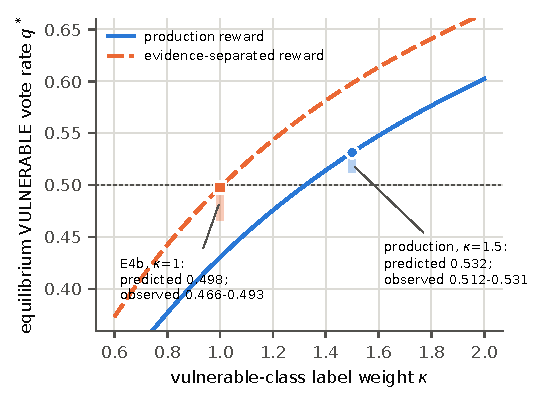
\includegraphics[width=\columnwidth]{fig_equilibrium.pdf}
\caption{Program A: closed-form equilibrium $q^*(\kappa)$ from Eq.~(\ref{eq:qstar}) for the production and evidence-separated rewards, with observed sampled-vote ranges (bars; 50-step bucket means, production steps $\ge$200). Values are recomputed from \texttt{reward\_counterfactuals.json}; the closed form reproduces the stored values to $10^{-9}$.}
\label{fig:eq}
\end{figure}

\textbf{E4b: fixing the reward fixes the behavior, not the discrimination.} A balanced reward (evidence-separated, $\kappa{=}1$, empty-set credit removed by emission gating) predicted $q^*\approx0.50$ and no emission collapse, with success pre-registered as $\Delta$AUC $\ge$ +0.03 against SFT-500. The behavioral predictions held (vote rate 49.25\% at steps 51--67, 45.35\% at the step-200 endpoint; correct-\vuln{} emission 99.98\%), and the efficacy endpoint failed: step-200 row AUC 0.5015 [0.4894, 0.5140], $\Delta$ vs.\ SFT-500 $-$0.0077 [$-$0.0253, +0.0096].

\textbf{Auxiliary routes.} Deployable predicted slicing was a registered no-go (AUC 0.510 vs.\ 0.529 for full functions on the forward 2021 holdout; $\Delta{=}-0.0186$ [$-0.0291$, $-0.0080$]); an oracle slice from ground-truth patch windows reaches 0.7485 [0.7312, 0.7657] but uses inference-unavailable information, a different protocol, and is a non-deployable bound. An evidence-first dense-supervision detector (E3) failed its registered early-stop gate (holdout AUC 0.4980 vs.\ matched classical 0.5293).

\textbf{Metrics.} \label{sec:metrics}
Pair metrics are shortcut-dominated: a character-length rule (``shorter is vulnerable'') attains 0.840 pair-AUC [0.819, 0.861] on VALID yet only 0.511 row AUC, and 73--84\% pair accuracy even among pairs with $<$5\% relative length difference (Fig.~\ref{fig:tg}b); the TF-IDF model attains 0.737 pair-AUC but 0.570 row AUC. Pair-grouped five-fold CV within TRAIN (64.45\% accuracy) overstates chronological VALID accuracy (55.3\%) by about 9 points. We therefore report row AUC.

\begin{figure*}[t]
\centering
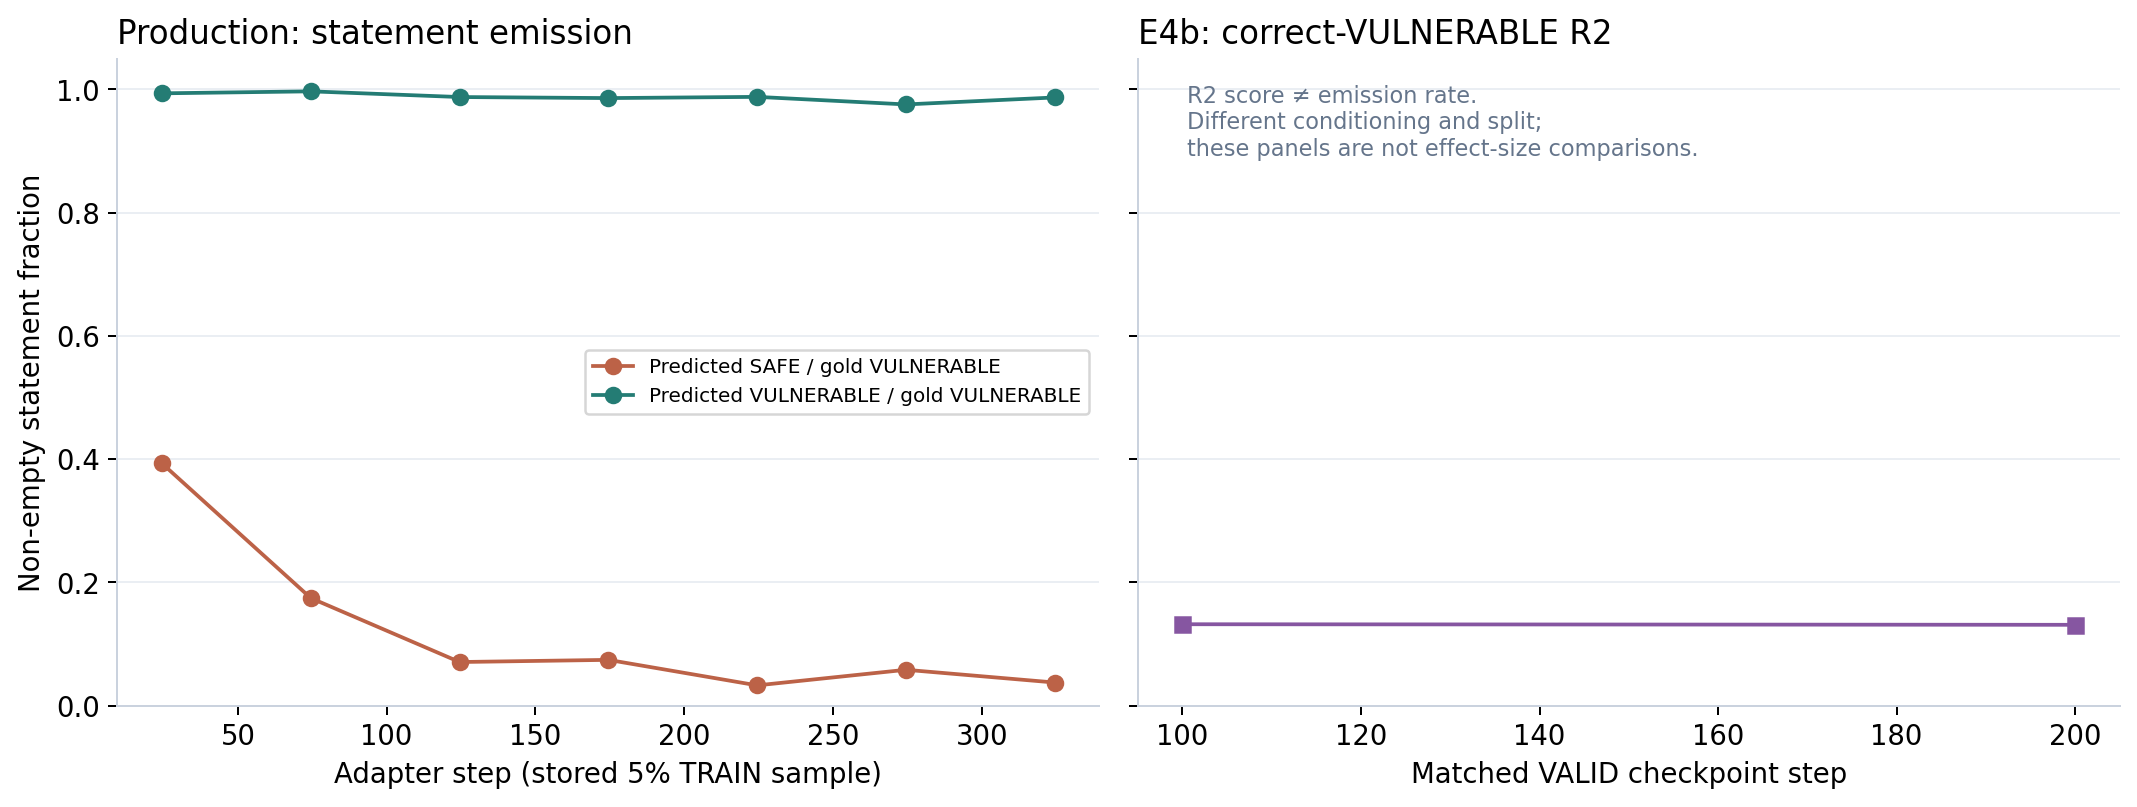
\includegraphics[width=0.62\textwidth]{tg_04_emission_collapse.png}\hfill
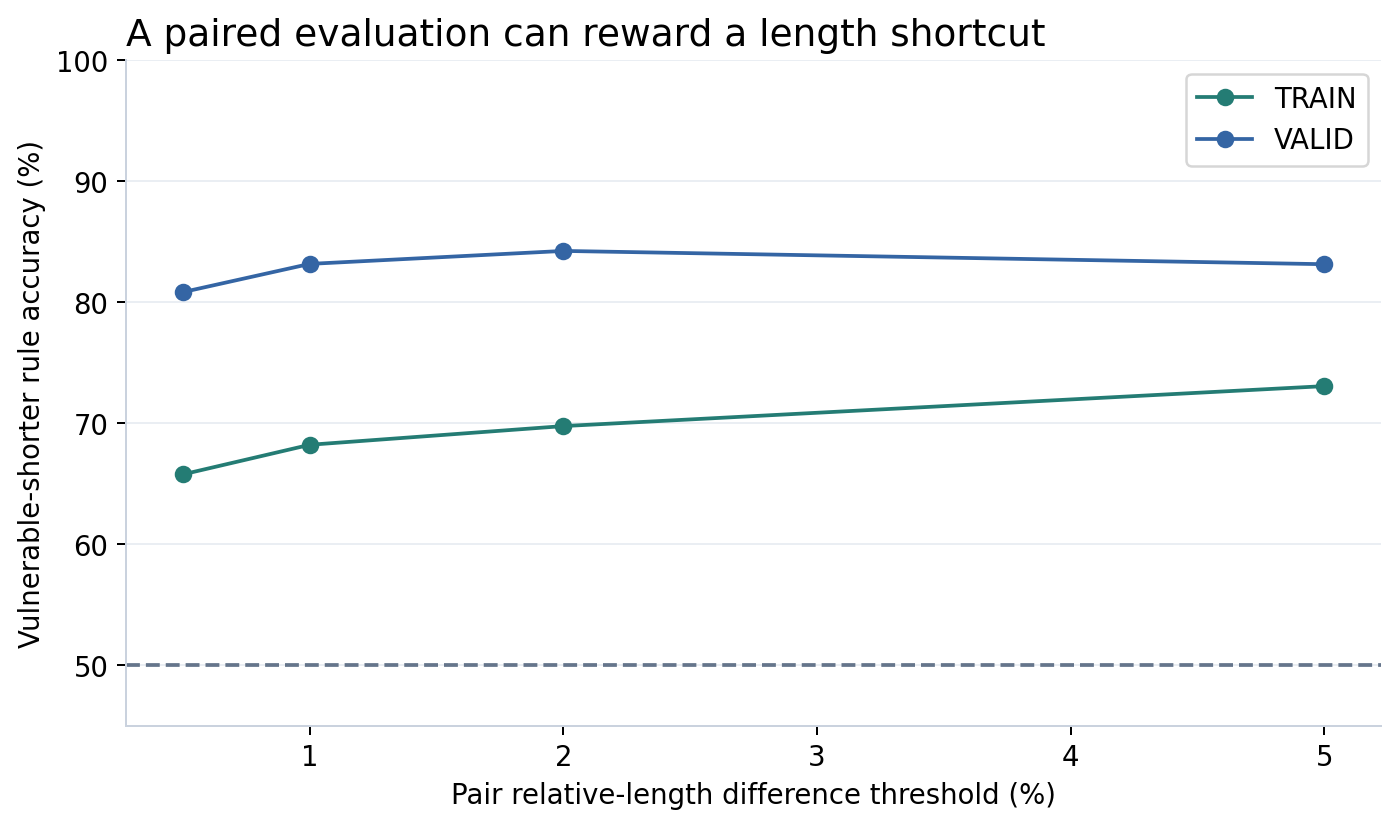
\includegraphics[width=0.35\textwidth]{tg_07_pair_length_shortcut.png}
\caption{Program A (figures from the TraceGRPO record). (a) Production: non-empty statement emission when the gold class is vulnerable, split by predicted verdict---emission on \safe{} predictions collapses while emission on correct-\vuln{} predictions stays near 1 (right panel: E4b correct-\vuln{} R2, a different quantity). (b) The ``vulnerable-shorter'' rule on near-length-matched pairs stays far above 50\%.}
\label{fig:tg}
\end{figure*}

\textbf{Blinded LLM-judge audit.} A 150-card deck (75 production-GRPO outputs, 75 classical outputs; balanced by gold label and correctness; one LLM judge, not a human) flagged 56/75 (74.7\%) of GRPO-324 rationales as post-hoc rationalization and 23/75 (30.7\%) as asserting at least one code claim absent from the function. Cross-system differences on localization and trace grades are not established (intervals include zero); rates describe the designed sample, not natural prevalence.

\textbf{Final single-read TEST} (2,526 rows / 1,263 pairs; 8 samples/row, T=0.8, seed 42) is in Table~\ref{tab:test}. Only the classical TF-IDF pipeline's accuracy interval excludes 50\%. Production GRPO's reward-induced prior tilt is visible out of sample as an extreme per-class split (18.1\% \safe{} / 82.3\% \vuln{} accuracy) that AUC correctly ignores. Neural-minus-classical paired $\Delta$AUC: SFT $-$0.0142 [$-$0.0278, $-$0.0004]; GRPO $-$0.0107 [$-$0.0249, +0.0038]; E4b $-$0.0135 [$-$0.0280, +0.0008]. Trace validity R3 is unavailable on TEST (0/1,263 vulnerable rows had eligible cached graph artifacts) and is reported as N/A, not zero. The classical model's own VALID$\to$TEST AUC decays from 0.570 to 0.531.

\begin{table}[t]
\centering\scriptsize\setlength{\tabcolsep}{2.5pt}
\caption{Program A: final TEST, single read. Accuracy with Wilson 95\% interval; row AUC with pair-cluster 95\% CI.}
\label{tab:test}
\begin{tabular}{lccc}
\toprule
System & Accuracy & Row AUC & \safe{} / \vuln{} acc.\\
\midrule
Classical & 52.5 [50.6, 54.5] & 0.531 [.524, .537] & 52.9 / 52.2\\
SFT-500 & 51.6 [49.7, 53.6] & 0.517 [.504, .529] & 56.8 / 46.5\\
GRPO-324 & 50.2 [48.3, 52.2] & 0.520 [.507, .533] & 18.1 / 82.3\\
E4b-200 & 51.4 [49.4, 53.3] & 0.517 [.504, .530] & 41.7 / 61.0\\
\bottomrule
\end{tabular}
\end{table}

\section{Program B: VulnGuard}
\label{sec:programB}
\subsection{Design and pre-registration}
The study was frozen on 2026-09-24 04:53 UTC. The primary contrast is GOLD versus PERMUTED. PERMUTED computes the same gold content values on the model's own sampled responses and then shuffles them among valid rollouts within each 16-rollout vulnerable+patched pair group; the reward-value multiset is preserved within each group, format reward stays on its originating output, and invalid outputs keep zero content. GOLD and PERMUTED share machinery, data, prompts, initialization, optimizer, seed pairing and evaluation, so the intended intervention is only whether the content value stays attached to its own response. BINARY (verdict-only, not evidence-conditioned) and FLIPPED (inverted gold) are secondary arms and manipulation checks.

The primary endpoint is strict localized \pc{} on the PrimeVul time-split test set: for each pair, sample $j$ of the vulnerable function is paired with sample $j$ of the patched one, and the joint is a success iff the vulnerable output earns full gold evidence (verdict \vuln{} plus a hit on an anchor line) \emph{and} the patched output is a valid \safe{} verdict (8 samples/function, T=0.6, top-p=0.95, $\le$640 tokens). The smallest effect of interest is 3.0\,pp; the pre-registered minimum detectable effect is 1.0--1.5\,pp. Invalid outputs are never coerced to \safe{}.

\subsection{Gold collapses; every historical rescue fails}
The first gold run (Qwen3-4B-Instruct-2507, seed 0) collapsed to always-\safe{}: the \vuln{} verdict rate fell from 0.68 to 0.00 by step 19--28 with validity at 1.0, mean content reward locked at exactly 0.500, and localization hit-rate 0. A sequence of fixes was pre-registered and tried, each tested before deployment: pair-grouped advantages (A1) collapsed again at the step-40 gate (mean \vuln{} rate 0.109); static side-balanced reward scaling with $k{=}3.553$ (C2) collapsed with the same mean; an EMA-centered baseline (A3) failed its own CPU toy-GRPO test and was never run on a GPU. Under the pre-registered cap of two automatic fixes, the study pivoted to a negative-result framing on 2026-09-24 16:23 UTC. Subsequent ablations (standardized, unstandardized, and CAPO-style post-normalization advantages~\cite{rlfourhs}) also failed to reverse the collapse; a machine-checked derivation showed the CAPO rescaling cancels exactly only for per-prompt, class-homogeneous groups, not for the mixed pair groups used here.

Replications on other backbones collapsed faster: Llama-3.2-3B at step 8, Qwen3-8B at 12, Qwen3-4B (hybrid) at 14, versus 18 for the reference run. (The Qwen3-8B run was stopped at step 30 by a low-entropy rule whose trigger condition was already true at the base model, so its stop was structurally guaranteed; the verdict-fraction collapse call is unaffected.) Gemma-4-E4B was infeasible: a vLLM/TRL native-LoRA synchronization gap of $\sim$13 nats ($130\times$ the gate) from step 1 is an infrastructure incompatibility, not a result.

\subsection{Base discrimination is near zero}
Discrimination $D=P(\vuln\mid\text{vulnerable input})-P(\vuln\mid\text{patched input})$ for the five untrained backbones is Qwen3-4B-2507 +0.036 [$-$0.003, +0.075], Llama-3.2-3B $-$0.014 [$-$0.059, +0.031], Qwen3-8B $-$0.017 [$-$0.065, +0.030], Qwen3-4B-hybrid $-$0.015 [$-$0.060, +0.030] and Gemma-4-E4B +0.032 [$-$0.012, +0.076]; none reaches the pre-registered +0.10 capability threshold and the estimates are mutually consistent (Cochran's $Q{=}6.15$, 4 df, $p{=}0.19$; pooled +0.007). The project first read this as a property of current open models and then \emph{withdrew} that reading on 2026-09-29 (Section~\ref{sec:corrections}): $D\approx0$ is equally consistent with weak discrimination, patched-side label problems, or a task-definition mismatch, because the prompt asks about \emph{any} vulnerability while the label reflects only the targeted fix. Base verdict rates on VAL are 78.4\% \vuln{} on vulnerable and 74.8\% on patched inputs, so an initially \safe{}-biased prior does not explain the collapse.

An H3 audit computed $D$ on VAL and PairVul-test for 15 checkpoints. Seven were scoreable and all have $D\le0.079$ (Table~\ref{tab:h3}). The eight gold-trained checkpoints failed with a \texttt{ZeroDivisionError}; we trace the cause in Section~\ref{sec:corrections}: they emit \emph{no} \vuln{} verdict on vulnerable inputs, with 100\% valid format.

\begin{table}[t]
\centering\footnotesize\setlength{\tabcolsep}{4pt}
\caption{Program B: audited discrimination $D$ (seven scoreable checkpoints); all below the +0.10 gate.}
\label{tab:h3}
\begin{tabular}{lcc}
\toprule
Checkpoint & $D$ (VAL) & $D$ (PairVul)\\
\midrule
base Qwen3-4B-2507 & +0.036 & +0.023\\
base Llama-3.2-3B & $-$0.014 & +0.007\\
BINARY s0 & +0.040 & +0.036\\
PERMUTED s0 & +0.079 & +0.043\\
PERMUTED s2 & +0.017 & +0.017\\
PERMUTED s3 & +0.020 & +0.026\\
PERMUTED s4 & $-$0.008 & $-$0.002\\
8 gold-trained & \multicolumn{2}{c}{no \vuln{} verdicts on vulnerable inputs}\\
\bottomrule
\end{tabular}
\end{table}

\subsection{The final matched cohort: 3 gold + 3 permuted seeds}
After the historical outcomes were known, the project froze a new, fully attested cohort: GOLD and PERMUTED, seeds 2, 3, 4, 40 optimizer steps each (a disclosed 40-step extension of a 110-step plan), final-step adapter chosen by fixed rule. Collapse stopping was log-only in this cohort. Training trajectories (Fig.~\ref{fig:vgtraj}a) diverge by step 15: all three GOLD runs fall to a \vuln{} verdict rate $\approx0$, while all three PERMUTED runs drift toward 1.

\begin{figure*}[t]
\centering
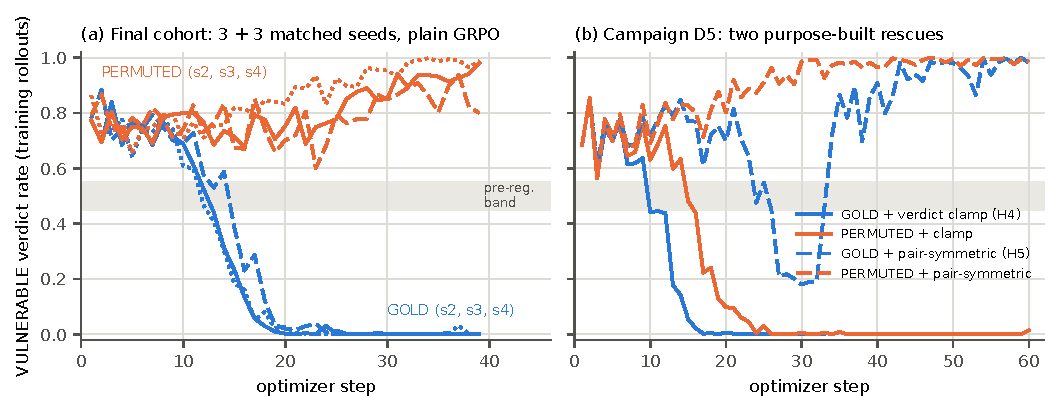
\includegraphics[width=\textwidth]{fig_vg_trajectories.pdf}
\caption{Program B: \vuln{} verdict rate over training. (a) Final cohort (3+3 matched seeds; step 40 has no logged rollout file and is omitted, not imputed). (b) Campaign D5 stage-1 runs: GOLD (blue) and PERMUTED (orange) under the verdict-rate clamp (solid) and the pair-symmetric reward (dashed). The shaded band is the pre-registered $[0.45,0.55]$ target; no run holds it.}
\label{fig:vgtraj}
\end{figure*}

Held-out endpoints (416 pairs, 3,328 samples per side per seed; Table~\ref{tab:cohort}) show the same split. GOLD answers \safe{} on essentially everything (100\% patched accuracy, 0.00--0.18\% vulnerable accuracy); PERMUTED answers \vuln{} on 85.6--98.8\% of vulnerable and 84.9--98.8\% of patched inputs. Balanced accuracy is $0.500$ for GOLD and 0.499--0.504 for PERMUTED; the strict endpoint is near zero in both arms. The CVE-clustered bootstrap (10{,}000 resamples, 381 clusters, matched seeds averaged within pair first) puts GOLD$-$PERMUTED at $-1.04$\,pp, 95\% CI [$-1.52$, $-0.62$], descriptive 90\% CI [$-1.43$, $-0.69$]. Pair-wise, PERMUTED beats GOLD on 41 pairs, GOLD beats PERMUTED on 1, and 374 tie.

\begin{table*}[t]
\centering\footnotesize\setlength{\tabcolsep}{4pt}
\caption{Program B: final-cohort held-out results (416 test pairs; 8 samples/function; 3,328 samples per side). TP/FP/TN/FN use valid predictions only (positive = \vuln{}). $P(\vuln|\cdot)$ is the verdict rate on vulnerable inputs / patched inputs.}
\label{tab:cohort}
\begin{tabular}{lcccccccc}
\toprule
Run & valid fmt & $P(\vuln|V)$ & $P(\vuln|P)$ & bal.\ acc. & TP/FP/TN/FN & evid.\ rate & \pc{} & pairs $\ge$1 success\\
\midrule
GOLD s2 & 1.0000 & 0.0000 & 0.0000 & 0.5000 & 0/0/3328/3328 & 0.0000 & 0.0000 & 0\\
GOLD s3 & 1.0000 & 0.0000 & 0.0000 & 0.5000 & 0/0/3328/3328 & 0.0000 & 0.0000 & 0\\
GOLD s4 & 1.0000 & 0.0018 & 0.0000 & 0.5009 & 6/0/3328/3322 & 0.0018 & 0.0018 & 1\\
PERM s2 & 0.9976 & 0.9669 & 0.9654 & 0.5000 & 3218/3213/110/99 & 0.2677 & 0.0066 & 16\\
PERM s3 & 1.0000 & 0.8561 & 0.8486 & 0.5038 & 2849/2824/504/479 & 0.2575 & 0.0237 & 27\\
PERM s4 & 0.9980 & 0.9877 & 0.9880 & 0.4986 & 3287/3288/32/36 & 0.4243 & 0.0027 & 3\\
\midrule
GOLD mean & --- & 0.0006 & 0.0000 & 0.5003 & --- & 0.0006 & 0.0006 & ---\\
PERM mean & --- & 0.9369 & 0.9340 & 0.5008 & --- & 0.3165 & 0.0110 & ---\\
\bottomrule
\end{tabular}
\end{table*}

\textbf{Neither arm beats the untrained base.} On the same 416 test pairs and protocol, the untrained base reaches \pc{} 4.30\% (balanced accuracy 0.476, valid-format rate 0.927), above every fresh arm (Fig.~\ref{fig:pc1}); the historical PERMUTED and BINARY arms (5.53\%, 5.32\%) are also near that level, GOLD (0.18\%, 0.12\%) and FLIPPED (0.21\%) are not. The pre-registered contrast H2 (PERMUTED$-$base $>$0) is therefore not met in the fresh cohort. We report this as descriptive: the frozen plan classifies the cohort as a post-hoc 40-step extension whose formal confirmatory test is pending a human-validation gate that was never completed, and no p-values or Holm decisions are used.

\begin{figure}[t]
\centering
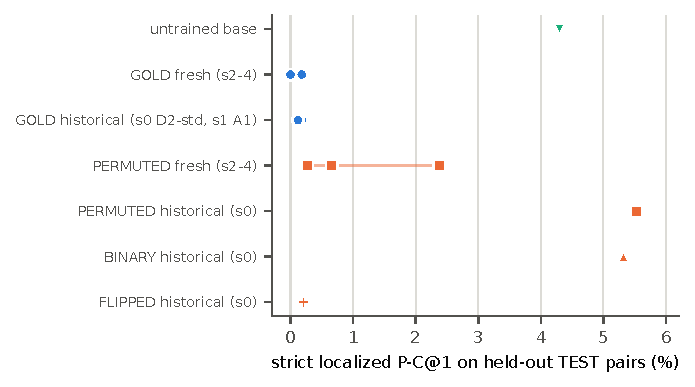
\includegraphics[width=\columnwidth]{fig_pc1_endpoints.pdf}
\caption{Program B: strict localized \pc{} on the 416 held-out test pairs, per condition (one marker per run). The untrained base exceeds every fresh GOLD and PERMUTED run.}
\label{fig:pc1}
\end{figure}

\subsection{Campaign D5: two purpose-built rescues}
\label{sec:d5}
After the baseline negative result, two mechanisms designed specifically against collapse were pre-registered, forecast, and witnessed (commit hash + SHA-256 externally timestamped) before the runs that test them.

\textbf{H4, verdict-rate clamp.} A Constrained-GRPO-style dual ascent~\cite{constrained} holds the \vuln{} and \safe{} verdict rates in $[0.45,0.55]$: with $C_1{=}\mathbb 1[\vuln]$, $C_2{=}\mathbb 1[\safe]$, dual variables $\lambda_k\leftarrow\max(0,\lambda_k+\eta(\text{rate}_k-d_k))$, $d_k{=}0.55$, $\eta{=}0.2$ (chosen on synthetic dynamics, never tuned on a real run), the advantage becomes $A_i=Z_{R,i}-\lambda_1 Z_{C_1,i}-\lambda_2 Z_{C_2,i}$ with $Z$ the within-group standardization. This is the simpler independent dual-ascent form that~\cite{constrained} describes as the typical background approach, not its softmax-simplex mechanism; the deviation was logged.

\textbf{H5, pair-symmetric reward.} Each rollout's reward is its own gold correctness multiplied by the \emph{other} side's group success rate (0 if the other side has no valid rollouts), removing the single-verdict escape.

\textbf{Outcome (60 planned steps, one gold and one permuted run per scheme).} All four runs end in a degenerate corner with near-zero pair correctness (Table~\ref{tab:d5}, Fig.~\ref{fig:vgtraj}b). S1a (gold, clamp) was halted by the watchdog at step 33; S1b (permuted, clamp) ran all 60 steps without triggering it yet reached the identical end state---not triggering an early-stop heuristic is not evidence against collapse. The pair-symmetric runs collapse to the \emph{opposite} corner (VAL \vuln{} rate 0.977 and 0.972); S1c briefly recovered toward balance around steps 26--31 (rate 0.19--0.45) before climbing back to 0.86--1.00 over its last ten steps. Scored against gates frozen before the runs: H4 $\to$ \texttt{H4\_DISABLED}; H5 $\to$ \texttt{H5\_DISABLED}, classified \texttt{H5\_NO\_RESCUE}, which closes this rescue family under the campaign's own decision tree.

\begin{table}[t]
\centering\scriptsize\setlength{\tabcolsep}{2.5pt}
\caption{Program B, Campaign D5 stage 1 (held-out VAL). $^{*}$halted by the watchdog; others ran the planned 60 steps. clamp = verdict-rate clamp (H4); pair = pair-symmetric reward (H5).}
\label{tab:d5}
\begin{tabular}{llccc}
\toprule
Run (scheme / arm) & End state & \vuln{} rate & \pc{} & Steps\\
\midrule
S1a clamp/gold & \safe{} corner & 0.000 & 0.000 & 33$^{*}$\\
S1b clamp/perm. & \safe{} corner & 0.002 & 0.000 & 60\\
S1c pair/gold & \vuln{} corner & 0.977 & 0.003 & 60\\
S1d pair/perm. & \vuln{} corner & 0.972 & 0.006 & 60\\
\bottomrule
\end{tabular}
\end{table}

\textbf{Why the clamp fails.} The implementation is correct: seven deterministic tests against the live trainer source confirm the dual variable's sign on both branches, its floor at zero, its one-step lag and that the advantage term is never detached. The failure is structural (Fig.~\ref{fig:h4}): (i) the content reward climbs to and locks at exactly 0.500, the value of an always-\safe{} policy on a half-patched population (Section~\ref{sec:geometry}); (ii) $\lambda_2$ rises correctly, from 0.06 at collapse onset (step 13) to 1.81 (S1a) and 3.77 (S1b), with no visible effect on the verdict rate; (iii) the cost term is a within-group standardized quantity, so once a group has collapsed to a single verdict its cost has zero variance and standardizes to \emph{exactly zero} regardless of $\lambda$; (iv) entropy falls from 0.51 to $<$0.02 and completion length from $\sim$247 to 21 tokens, leaving little gradient headroom. We classify the result as \texttt{CONSTRAINT\_CONFLICTS\_WITH\_REWARD\_GRADIENT} with the zero-variance gap as an independently verified, compounding limitation. Whether the softmax-simplex form or a non-group-relative cost estimator shares the failure is untested; the planned reward-vs-constraint gradient-norm audit was deferred and not run.

\begin{figure*}[t]
\centering
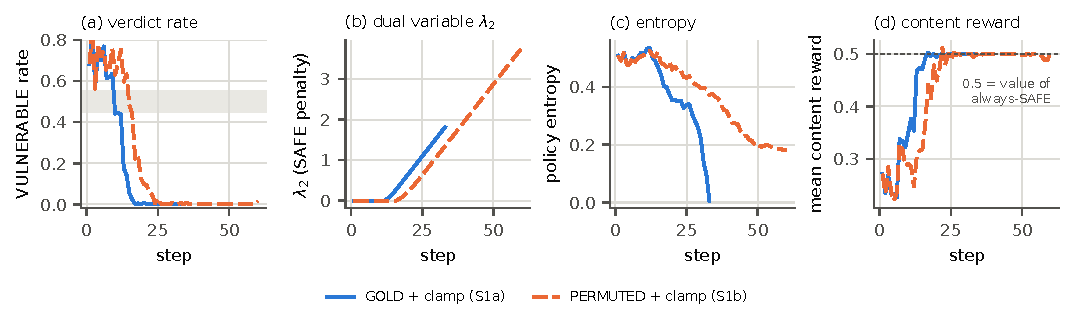
\includegraphics[width=\textwidth]{fig_h4_mechanism.pdf}
\caption{Program B: clamp mechanism, S1a (gold, solid; halted at step 33) and S1b (permuted, dashed). (a) Verdict rate crashes through the target band; (b) the SAFE-side dual variable grows monotonically; (c) policy entropy collapses; (d) content reward locks at 0.5.}
\label{fig:h4}
\end{figure*}

\subsection{Controls and judge calibration}
\textbf{Positive control.} A deliberately easy, symmetric marker task (512 train / 100 held-out functions with an inert marker A or B at the same line, 40 steps, one seed, same stack) took held-out balanced accuracy from 0.960 to 1.000 and strict pair-correctness from 0.8625 to 1.000. Its pre-registered status is \texttt{BASE\_CEILING\_LIMITED}, not success, because the base started near ceiling. It argues against a universally broken trainer; it does not show that the asymmetric vulnerability reward is the only difference.

\textbf{Gradient audit.} A fixed-batch audit (16 pairs, 128 rollouts per side) found a patched/vulnerable gradient-norm ratio of 1.076 (descriptive range [0.675, 1.957]) and near-zero cross-side cosine ($-0.090$); the policy-effect readout saturated. Simple patched-gradient dominance is not supported; no causal gradient conclusion is drawn.

\textbf{Judge calibration.} A judge that flags 46/50 designated-bad and 1/50 designated-good NIST Juliet functions (92\%/2\%) flags 47.6\% (LIKELY+POSSIBLY, $n{=}115$) of real, era-matched C functions from the same projects under an open ``find any vulnerability'' prompt. The 115 functions were checked only against fix-touched files in the project's own pool, so some may carry untracked vulnerabilities; the $\sim$46-point gap nevertheless shows that a false-positive floor calibrated on synthetic code can badly underestimate the real-code floor. On \emph{patched} functions the same judge flags 82/144 parsed (56.9\%; 56/200 unparsed), a gap of 9.4\,pp over the real-code floor---a flag rate, not an established label-noise rate. Deterministic reward-vs-judge agreement is 226/270 (83.7\%), inflated by a floor effect on collapsed outputs. Human validation packets were prepared but zero human labels were ever entered.

\section{Cross-Program Synthesis}
\label{sec:synthesis}
\subsection{Every system lies on the no-discrimination diagonal}
Fig.~\ref{fig:roc} plots every held-out TEST system from both programs by $P(\vuln\mid\text{patched/\safe{} input})$ and $P(\vuln\mid\text{vulnerable input})$. A discriminating system lies above the diagonal. None does: the TraceGRPO neural systems and the TF-IDF baseline, the untrained base, four VulnGuard reward arms, and the extreme corners (GOLD at the origin, FLIPPED and PERMUTED at the top-right) all sit on or within sampling noise of it. RL moves a policy \emph{along} the diagonal---from the base's prior near 0.7, to 0.82 in production GRPO, to 0 in GOLD---without lifting it off. This is the quantity the verdict-rate figures in both programs are tracking, and it explains why accuracy at the argmax is a misleading endpoint: production GRPO's greedy split swung from 30\% to 64\% \vuln{} at chance accuracy, and in Program B balanced accuracy is 0.500 for GOLD and for PERMUTED despite opposite policies.

\begin{figure}[t]
\centering
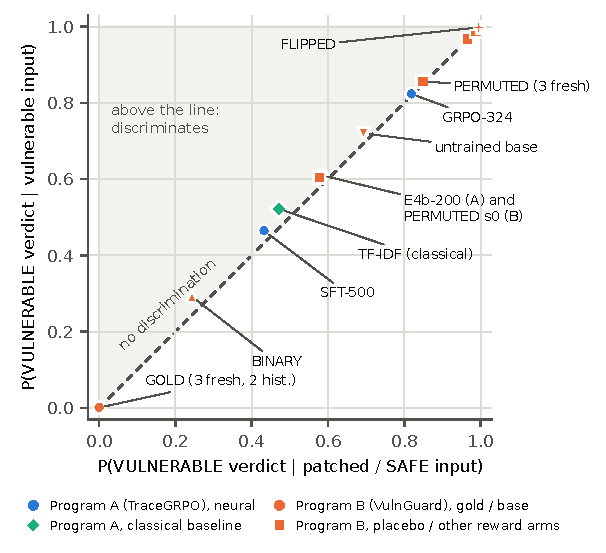
\includegraphics[width=\columnwidth]{fig_roc_space.pdf}
\caption{Both programs on one plot (held-out TEST sets; different aggregation: Program A uses its frozen 8-vote rule per row, Program B uses per-sample verdict rates). Dashed diagonal = no discrimination. Program B's three fresh GOLD runs, two historical GOLD runs and the PERMUTED runs overlap at the corners.}
\label{fig:roc}
\end{figure}

\subsection{Reward geometry of input-independent policies}
\label{sec:geometry}
The following statements are analytic consequences of the \emph{frozen reward definitions}; they are our derivations, checked against logged values where stated, not results from either original study. Consider a policy that emits \vuln{} with probability $q$ independent of the input, on a population that is half vulnerable and half patched.

\textbf{Gold (Program B).} Let $h$ be the probability that a \vuln{} verdict on a vulnerable function also hits an anchor line, so the gold success probability on a vulnerable function is $g_V=qh$, and on a patched function it is $1-q$. The expected content reward is $R(q)=\tfrac12(1-q)+\tfrac12 q\,h$, strictly decreasing in $q$ for $h<1$, with maximum $\tfrac12$ at $q{=}0$. This matches the logged plateau: content reward climbs to and locks at exactly 0.500. At step 1 of S1a the logged vulnerable-side success is $g_V{=}0.285$ and the overall \vuln{} rate is $q{=}0.684$; the formula gives $\tfrac12(0.316)+\tfrac12(0.285)=0.300$, and scaling by the valid-output fraction (0.896; invalid outputs earn zero content) gives 0.269 against a logged 0.271. The \safe{} side's correct answer requires no evidence, while the \vuln{} side's requires a localization hit; this asymmetry makes the always-\safe{} corner reward-dominant.

\textbf{Pair-symmetric (Program B).} With reward $=$ own correctness $\times$ other side's group success rate, a constant policy at either corner earns exactly 0 (the other side's success rate is 0 at both corners), while for interior $q$ the expected reward is proportional to $q(1-q)\,h$, maximal at $q{=}\tfrac12$. In expectation the reward therefore \emph{prefers} balance and is indifferent between the corners---yet S1c and S1d ended at the \vuln{} corner. Reward optimum at $q{=}\tfrac12$ is not sufficient: at a corner there is no restoring gradient, and the approach to it is a dynamics question (step size, standardization of sparse rewards) that we did not isolate.

\textbf{Constrained (Program B).} Each cost advantage is $\lambda_k(C_k-\bar C_g)/(\mathrm{sd}_g+\varepsilon)$ per group $g$; if every rollout in a group has the same verdict, $C_k-\bar C_g=0$ identically, so the term vanishes for any $\lambda_k$.

\textbf{Program A.} Eq.~(\ref{eq:qstar}) is the corresponding statement for a weighted five-component reward estimated from archived cells. The same asymmetry appears as the vacuous-credit convention (credit for \safe{} with no evidence), and the label multiplier $\kappa{=}1.5$ happens to offset it: $q^*{=}0.53$ in the production reward, versus $0.43$ at $\kappa{=}1$ and $0.498$ for the evidence-separated reward.

\textbf{Reading across.} In both programs a verifiable reward priced the classes unequally for an input-ignoring policy; the policy moved to where the price was favorable. In Program A the offset bounded the drift near $q^*\approx0.5$; in Program B no offset existed and the policy reached a corner. The cross-program contrast (interior versus corner) is, however, confounded with learning rate ($10^{-6}$--$5{\times}10^{-6}$ vs.\ $2{\times}10^{-5}$), initialization (SFT vs.\ base), number of steps, and output contract (Table~\ref{tab:programs}). We state it as a hypothesis, not a finding, and describe the test in Section~\ref{sec:discussion}.

\subsection{Corrections move the prior, not the capability}
In Program A, balancing the reward fixed the behavior to prediction yet left AUC at 0.5015. In Program B, a clamp designed to hold the prior in $[0.45,0.55]$ and a pair-symmetric reward designed to remove the single-verdict escape both failed to hold it, and neither produced discrimination. The shared moral is that stabilizing the verdict prior and creating input-conditional signal are different problems, and only the first is addressed by reward engineering when the starting policy is itself a weak discriminator (Program A: SFT-500 train probe 55\%, within-pair pool-vote AUC consistent with chance; Program B: base $D\approx0.03$).

\subsection{Metric lessons shared by both programs}
(i) Report rates by side: both programs' headline distortions are class-conditional. (ii) Threshold-free, row-level metrics (row AUC) and strict pair metrics measure different things: strict \pc{} is exactly zero for any single-verdict policy and positive for a noisy, non-discriminating one, so the untrained base's 4.30\% (with $D\approx0.03$) is not evidence of discrimination and must be read against an independent-sides null; pair-AUC is exploitable by length (0.84). (iii) Invalid outputs must be first-class outcomes, never coerced. (iv) Collapse must be diagnosed from continuous trajectories, not from a stop heuristic that did or did not fire.

\section{Discussion}
\label{sec:discussion}
\textbf{What the evidence supports.} Under chronological or time-ordered protocols, neither teacher-trace SFT nor verifiable-reward GRPO---with or without SFT initialization, with gold or placebo rewards, with or without purpose-built rescues---produced detectable vulnerability discrimination in a 3--8B model on these corpora; the TF-IDF baseline in Program A did, modestly (AUC 0.5307, only accuracy interval excluding chance, decaying from VALID). The reward-induced prior motion is predictable from the reward definitions.

\textbf{What it does not show.} It does not show that RL, reasoning supervision, slicing or neural detectors cannot work. Every policy started from $D\approx0$, so the studies cannot separate ``RL cannot create discrimination the base lacks'' from ``these specific rewards were insufficient''. Program B's primary endpoint is near zero in both arms, so the GOLD-vs-PERMUTED contrast measures \emph{which corner} each arm reached, not a useful-detection gap.

\textbf{A direct test of the interior-vs-corner hypothesis.} Because the two programs differ in many ways at once, the cleanest follow-up is a $2{\times}2$: Program B's gold reward at Program A's step size and SFT initialization, and Program A's $\kappa{=}1$ reward at Program B's step size from the base. A different reading of Program B's behavior---a random walk with absorbing corners, which the zero-information PERMUTED placebo would exhibit (it ended toward \vuln{} in 3/4 seeds, namely the three fresh ones, with the historical seed mid-range, and toward \safe{} in none)---would predict corner-reaching irrespective of reward asymmetry; the $2{\times}2$ distinguishes it as well. We did not run these experiments.

\textbf{What a positive result would likely require.} (a) An initialization with audited, input-conditional signal (supervised pair-contrastive training, or representation probing as a precondition) before RL; (b) reward suites audited for net per-group prior push and for credit that can be earned without evidence; (c) length-aware modeling where evidence density is $\sim$1\%; (d) row-level, threshold-free metrics with pair-cluster statistics as the reporting default.

\section{Threats to Validity and Corrections to Earlier Drafts}
\label{sec:corrections}
\textbf{Scope.} One corpus family (PrimeVul/SecVulEval/PairVul derivatives), C/C++ only, 3--8B models with LoRA, one prompt family per program, one GPU class. Program A's E3 is single-seed by pre-registered early stop; Program B's fresh cohort has three seeds per arm and its CI conditions on those seeds. Both programs' statistical power is limited: Program A detects $\Delta$AUC $\gtrsim0.03$ at 80\% power; Program B's MDE is 1.0--1.5\,pp.

\textbf{Test exposure and governance.} Program A's TEST was read once per registered system (with a post-inference aggregation fix that did not reopen TEST). Program B's historical runs were evaluated on the test split before the fresh cohort was frozen, which the frozen plan itself states weakens any ``untouched confirmatory'' claim; the 40-step cohort is a post-hoc extension, and human validation was never completed. Program B's fresh cohort ran from a dirty worktree (commit \texttt{1a7157e}); its source, config, dataset and adapter hashes are recorded, and \texttt{src/} was independently shown byte-identical to that commit.

\textbf{Judge and label validity.} Both audits use a single LLM judge (not human grading). Patched-side residual flaws and label noise remain unestablished.

\textbf{Compute accounting.} See Appendix~\ref{app:compute}; neither program has a certifiable total.

\textbf{Corrections found while merging the two records.} We list these because each appears in an earlier draft or summary and is contradicted by a raw artifact.
\begin{enumerate}
\item \emph{Cause of the H3 failures (VulnGuard draft).} The draft states that the eight gold checkpoints failed because they ``produced zero valid parses on one side.'' The failing statement is \texttt{hits / vul}, where \texttt{vul} counts valid \emph{\vuln{} verdicts} on vulnerable inputs. Fresh-cohort GOLD has valid-format rate 1.0000 and zero \vuln{} verdicts, so the denominator is zero because the policy never answers \vuln{}, not because outputs are invalid.
\item \emph{Label of the primary result.} Two VulnGuard summaries call $-1.04$\,pp a ``$\Delta D$''. The bootstrap file defines it as the difference in per-pair strict \pc{} (mean across matched seeds within pair); $D$ is $\approx0$ for every arm.
\item \emph{Fresh cohort omitted.} The VulnGuard manuscript draft's abstract and results never mention the 3+3 cohort, the PERMUTED drift toward \vuln{} (final-step rates 0.99/0.84/1.00), or the untrained-base comparison; the headline ``gold collapses, predominantly always-\safe{}'' is correct but incomplete.
\item \emph{Patched-audit rate.} The 56.9\% figure is a judge flag rate, as VulnGuard's own dossier stresses; it is not label noise, and it sits 9.4\,pp above the real-code floor.
\item \emph{Withdrawn claim.} The ``near-chance base discrimination is a property of current open models'' entry was withdrawn by the project on 2026-09-29; we do not make it.
\item \emph{TraceGRPO Figure 3.} The released ``reward equilibrium'' figure labels $q^*{=}0.4307$ as ``Production predicted''. That is the $\kappa{=}1$ value; production used $\kappa{=}1.5$ ($q^*{=}0.5315$). The cause is \texttt{build\_publication\_assets.py} line 79, which selects the first \texttt{closed\_form\_q\_star*} key. As drawn, the figure makes a successful prediction look like a miss; Fig.~\ref{fig:eq} here is recomputed from the source JSON.
\item \emph{Test-suite size and one abstract phrase (TraceGRPO draft).} The draft cites a 569-test suite; the preserved validation log shows 532 passed, and the repository has 459 \texttt{test\_} functions. We cite the log. The draft's abstract calls 50.18\% the ``best'' SFT accuracy, whereas run 1 reached 50.50\%; we report the range.
\end{enumerate}

\section{Conclusion}
Two independent, instrumented programs on one task agree: verifiable rewards verified what they rewarded---verdict-prior position and evidence emission---and not vulnerability discrimination. Program A explains the drift with a closed-form equilibrium and shows that fixing the reward fixes the behavior but not the capability; Program B shows that a gold reward is outperformed on the strict endpoint by a reward that has destroyed the signal and by the untrained base, and that two rescues designed for exactly this failure either fail or relocate it, one with an exact structural reason. Together they place the open problem upstream of reward engineering: obtaining a starting policy that carries input-conditional signal, and measuring it with endpoints that cannot be satisfied by moving a prior.

\appendices
\section{Claims Register}
\label{app:claims}
\textbf{Supported.} Corpus/split reproducibility from manifests (A); annotation coverage as reported (A); SFT learns format without transmitting discrimination in three variants (A); label learnability in isolation (A, C-L1); no established AUC gain from production or balanced GRPO (A); closed-form equilibrium reproduces stored values and predicts the vote-rate range (A); gold-reward collapse in all fresh and historical variants tested (B); permuted-reward drift toward \vuln{} in the fresh cohort (B); neither fresh arm exceeds the untrained base on strict \pc{} (B); both Campaign D5 rescues fail their frozen gates (B); the clamp's cost term is exactly zero for single-verdict groups (B); every evaluated system lies on the no-discrimination diagonal (A+B).

\textbf{Not claimed.} That RL improves vulnerability detection or beats classical methods; that all slicing fails or oracle slices are deployable; any multi-seed E3 claim; any step-400 production evaluation; that GOLD-vs-PERMUTED is a confirmatory test (human gate pending; post-hoc 40-step extension); that near-chance $D$ is a property of open models; that 56.9\% is label noise; that the interior-vs-corner difference between programs is caused by $\kappa$ (confounded); that the LLM-judge audits are human grading or natural prevalence; exact compute totals; novelty.

\section{Reproduction Notes}
\label{app:artifacts}
Program A: \url{huggingface.co/Dhruv1000/tracegrpo}; key files: \path{docs/MASTER_REPORT.md}, \path{results/phase10/final_test_20261012/test_final_metrics.json}, \path{results/phase6/review22/reward_counterfactuals.json}. Program B: \url{huggingface.co/datasets/Dhruv1000/vulnguard-code-and-report} (code, docs, \path{results/final_scientific_audit_20260927/}, \path{results/campaign_D5/}) and \url{huggingface.co/datasets/Dhruv1000/vulnguard-results} (large run artifacts; checkpoints in LFS archives). All new figures in this paper are produced by \path{figures_src/make_figures.py} from those files; Fig.~\ref{fig:tg} reuses figures from the TraceGRPO record.

\section{Pre-Registered Hypotheses of Program B}
H1: GOLD $>$ PERMUTED on \pc{} (one-sided CVE-cluster bootstrap lower bound $>0$ and Holm-adjusted sign-flip $p<.05$); H1-null: equivalence via TOST at 3.0\,pp; H2: PERMUTED $-$ base $>0$; H3: BINARY raises verdict accuracy relative to its \pc{} gain more than GOLD; H4: FLIPPED $<$ base (manipulation check); H5: GOLD$-$base P-Pass@$k$ gap shrinks with $k$; H6: base-trained probe transfers to GOLD with $\Delta$AUC $\le0.02$ or fails; H7: placebo gain on Llama $\approx0$. Holm family: \{H1, H2, H4, H1-Llama\}. The Campaign D5 hypotheses H4 (clamp) and H5 (pair-symmetric) are a separate numbering; of the larger D5 plan only H3, H4, H5 and H8 were run.

\section{Compute Accounting}
\label{app:compute}
Program A: identified subtotal 102.703 GPU/allocated-GPU hours (non-overlapping known entries); incomplete historical allocation means the true total is higher. Program B: the final-cohort controller queue recorded 11.82 GPU-job hours of training and 12.82 hours including evaluation; the earlier GPU-window summary header reports 47.7 GPU-hours at its 2026-10-02 snapshot, while its itemized rows sum to 39.7 hours. We do not reconcile these figures and make no total claim.

\section{Reference Verification Status}
Entries marked \emph{lit-table} resolved to the stated title and authors in the VulnGuard project's own audit (arXiv export API, 2026-09-23). Entries marked \emph{hf-index} were also found in the Hugging Face paper index while preparing this manuscript (existence only; the index does not hold every paper). Not found in that index and not independently verified here: arXiv:2507.03051 (lit-table verified earlier), 2306.17193, 2501.13291, 2602.05863, 2606.20502, 2608.09643, 2607.26656, 2602.10418, 2602.06687, 2601.10496, 2607.20543. Bibliography keys \path{secvuleval}, \path{semantictrap}, \path{vulagentrl}, \path{seccodeprm}, \path{rlfourhs}, \path{grpo}, \path{drgrpo}, \path{dapo} carry titles or authors from the project drafts or from memory and must be re-verified against primary sources before submission.

\bibliographystyle{IEEEtran}
\bibliography{references}

\end{document}
